\documentclass{VUMIFInfKursinis}
\usepackage{algorithmicx}
\usepackage{algorithm}
\usepackage{algpseudocode}
\usepackage{amsfonts}
\usepackage{amsmath}
\usepackage{bm}
\usepackage{color}
\usepackage{graphicx}
% \usepackage{hyperref}  % Nuorodų aktyvavimas
\usepackage{url}

\usepackage{acro}
\usepackage{tikz}
\usetikzlibrary{decorations.pathreplacing}


% Titulinio aprašas
\university{Vilniaus universitetas}
\faculty{Matematikos ir informatikos fakultetas}
\institute{Informatikos institutas}  % Užkomentavus šią eilutę - institutas neįtraukiamas į titulinį
\department{Programų sistemų katedra}
\papertype{Kursinis darbas}
\title{Medžiagų maišymo modeliavimas cheminėse
reakcijose}
\titleineng{Modelling the mixing of reagents in
chemical reactions}
\status{4 kurso 3 grupės studentas}
\author{Arnas Vaicekauskas}
% \secondauthor{Vardonis Pavardonis}   % Pridėti antrą autorių
\supervisor{Asist. Dr. Rokas Astrauskas}
\date{Vilnius \\ \the\year}

% Nustatymai
% \setmainfont{Palemonas}   % Pakeisti teksto šriftą į Palemonas (turi būti įdiegtas sistemoje)
\bibliography{bibliografija} 

\DeclareAcronym{yag}{
    short   = YAG,
    long    = Itrio aliuminio granatas    
}

\begin{document}
\maketitle

\tableofcontents

\sectionnonum{Sąvokų apibrėžimai}

% Sutartinių ženklų, simbolių, vienetų ir terminų sutrumpinimų sąrašas (jeigu
% ženklų, simbolių, vienetų ir terminų bendras skaičius didesnis nei 10 ir
% kiekvienas iš jų tekste kartojasi daugiau nei 3 kartus).

\sectionnonum{Įvadas}
% Įvade apibūdinamas darbo tikslas, temos aktualumas ir siekiami rezultatai.

% Iš panašių darbų atrodo, kad įvadą sudaro
%
%
%

% Dalykai, kurie gali įeiti į tikslą:
% - Literatūros apžvalga (skamba labiau kaip užduotis, negu tikslo dalis)
% - Sukurti patobulintą kompiuterinį modelį iš matematinio modelio 
% - Ištirti maišymą (statistinė optimalaus maišymo paieška kai B = 2n, n > 1)
% - Rasti optimalų maišymo laiką,
Šio \textbf{darbo tikslas} yra patobulinti egzistuojantį matematinį itrio aliuminio granato (\acs{yag}) reakcijos modelį 
\cite{mackeviciusCloserLookComputer2012} įtraukiant medžiagų maišymo procesą.

Iškelti darbo uždaviniai:

\begin{enumerate}
\item Sudaryti dviejų dimensijų skaitinį \ac{yag} medžiagos reakcijos modelį Dekarto koordinačių sistemoje
\item Sudaryti kompiuterinį modelį pagal skaitinį modelį
\item Patikrinti kompiuterinio modelio teisingumą ir palyginti gautus rezultatus su eksperimentiniais
\item Sukurti skaitinį medžiagų maišymo proceso modelį 
\item Papildyti kompiuterinį modelį išmaišymo procesu
\item Ištirti reakcijos pabaigos laiko priklausomybę nuo išmaišymo laiko
\end{enumerate}

% Užduotyse paminėti
% - Maišymo modelio kūrimas
% - Modelio tikslumo užtikrinimas
% - 
% - 

% \section{Pagrindinė tiriamoji dalis}
% Pagrindinėje tiriamojoje dalyje aptariama ir pagrindžiama tyrimo metodika;
% pagal atitinkamas darbo dalis, nuosekliai, panaudojant lyginamosios analizės,
% klasifikacijos, sisteminimo metodus bei apibendrinimus, dėstoma sukaupta ir
% išanalizuota medžiaga.
%

% \subsection{Poskyris}

\section{Skaitinis modelis}

\subsection{Erdvės diskretizavimas Dekarto koordinačių sistemoje}

Dviejų dimensijų skaitiniam modeliui erdvė buvo padalinta į $N \times M$ taškų 
nutolusių vienas nuo kito fiksuotais $\Delta x$ ir $\Delta y$ atstumais.

\begin{figure}[!h]
\centering
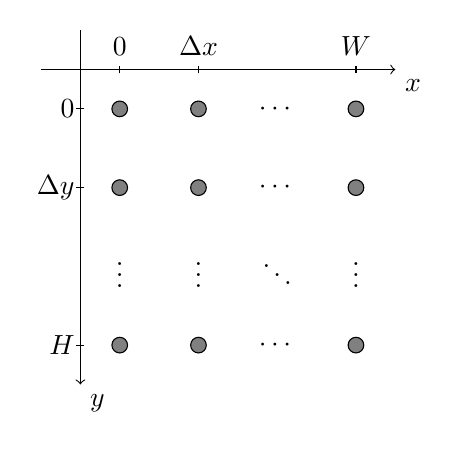
\begin{tikzpicture}

   % Set up styles for the grid
  \tikzset{
      node/.style={circle, draw, fill=gray, inner sep=2pt},
      ellipsis/.style={draw=none, fill=none}
  }

  \draw[->] (0, -0.5) -- (4.5, -0.5) node[anchor=north west] {$x$};  % x-axis
  % x-axis ticks
  \draw[-] (1, -0.55) -- (1, -0.45) node[anchor=south] {$0$};
  \draw[-] (2, -0.55) -- (2, -0.45) node[anchor=south] {$\Delta x$};
  \draw[-] (4, -0.55) -- (4, -0.45) node[anchor=south] {$W$};
  
  \draw[<-] (0.5,-4.5) node[anchor=north west] {$y$} -- (0.5, 0);  % y-axis
  % y-axis ticks
  \draw[-] (0.45, -1) -- (0.55, -1) node[anchor=east] {$0$};
  \draw[-] (0.45, -2) -- (0.55, -2) node[anchor=east] {$\Delta y$};
  \draw[-] (0.45, -4) -- (0.55, -4) node[anchor=east] {$H$};


  % Draw the 3x3 grid of colored circles in a 4x4 layout
  \foreach \x in {1, 2, 4} {
      \foreach \y in {1, 2, 4} {
          \node[node] at (\x, -\y) {};
      }
  }

  % Add ellipses in the 4th row and column for continuation

  \node[ellipsis] at (3, -1) {$\cdots$};
  \node[ellipsis] at (3, -2) {$\cdots$};
  \node[ellipsis] at (3, -4) {$\cdots$};

  \node[ellipsis] at (1, -3) {$\vdots$};
  \node[ellipsis] at (2, -3) {$\vdots$};
  \node[ellipsis] at (4, -3) {$\vdots$};

  \node[ellipsis] at (3, -3) {$\ddots$};

\end{tikzpicture}
\caption{ diskretizuota erdvė }
\end{figure}

Čia 

\subsection{Dviejų dimensijų skaitinis modelis Dekarto koordinačių sistemoje}

% \subsubsection{Skirsnis}
% \subsubsubsection{Straipsnis}
% \subsubsection{Skirsnis}
% \section{Skyrius}
% \subsection{Poskyris}
% \subsection{Poskyris}

\sectionnonum{Rezultatai ir išvados}
% Išvadose ir pasiūlymuose, nekartojant atskirų dalių apibendrinimų,
% suformuluojamos svarbiausios darbo išvados, rekomendacijos bei pasiūlymai.

\printbibliography[heading=bibintoc] % Literatūros šaltiniai aprašomi
% bibliografija.bib faile. Šaltinių sąraše nurodoma panaudota literatūra,
% kitokie šaltiniai. Abėcėlės tvarka išdėstoma tik darbe panaudotų (cituotų,
% perfrazuotų ar bent paminėtų) mokslo leidinių, kitokių publikacijų
% bibliografiniai aprašai (šiuo punktu pasirūpina LaTeX). Aprašai pateikiami
% netransliteruoti.

\appendix  % Priedai
% Prieduose gali būti pateikiama pagalbinė, ypač darbo autoriaus savarankiškai
% parengta, medžiaga. Savarankiški priedai gali būti pateikiami kompiuterio
% diskelyje ar kompaktiniame diske. Priedai taip pat vadinami ir numeruojami.
% Tekstas su priedais siejamas nuorodomis (pvz.: \ref{img:mlp}).

% \section{Neuroninio tinklo struktūra}
% \begin{figure}[H]
%     \centering
%     \includegraphics[scale=0.5]{img/MLP}
%     \caption{Paveikslėlio pavyzdys}   % Antraštė įterpiama po paveikslėlio
%     \label{img:mlp}
% \end{figure}


% \section{Eksperimentinio palyginimo rezultatai}
% % tablesgenerator.com - converts calculators (e.g. excel) tables to LaTeX
% \begin{table}[H]\footnotesize
%   \centering
%   \caption{Lentelės pavyzdys}    % Antraštė įterpiama prieš lentelę
%   {\begin{tabular}{|l|c|c|} \hline
%     Algoritmas & $\bar{x}$ & $\sigma^{2}$ \\
%     \hline
%     Algoritmas A  & 1.6335    & 0.5584       \\
%     Algoritmas B  & 1.7395    & 0.5647       \\
%     \hline
%   \end{tabular}}
%   \label{tab:table example}
% \end{table}

\end{document}
